%%%%%%%%%%%%%%%%%%%%%%%%%%%%%%%%%%%%%%%%%%%%%%%%%%%%%%%%%%%%%%%%%%%%%%%%%%%%%% 
\section {Muon decays in flight and the degrader thickness}

{\red Briefly Describe the multistage simulation - standard Mu2e scheme
  \begin{itemize}
  \item
    first: simulation of muon beam till the DS
  \item
    then - resampling in the DS, simulaiton of the muon decays in flight
  \item
    Krzysztof's scheme - constant weight factor, but a change in the Z distributions
    of the muon decay vertices
  \end{itemize}
}


%%%%%%%%%%%%%%%%%%%%%%%%%%%%%%%%%%%%%%%%%%%%%%%%%%%%%%%%%%%%%%%%%%%%%%%%%%%%%%
\subsection {Constraining the muon proper decay time - validation}

\begin{figure}[H]
  \begin{tikzpicture}
    \node[anchor=south west,inner sep=0] at (0,0.) {
      % \node[shift={(0 cm,0.cm)},inner sep=0,rotate={90}] at (0,0) {}
      \makebox[\textwidth][c] {
        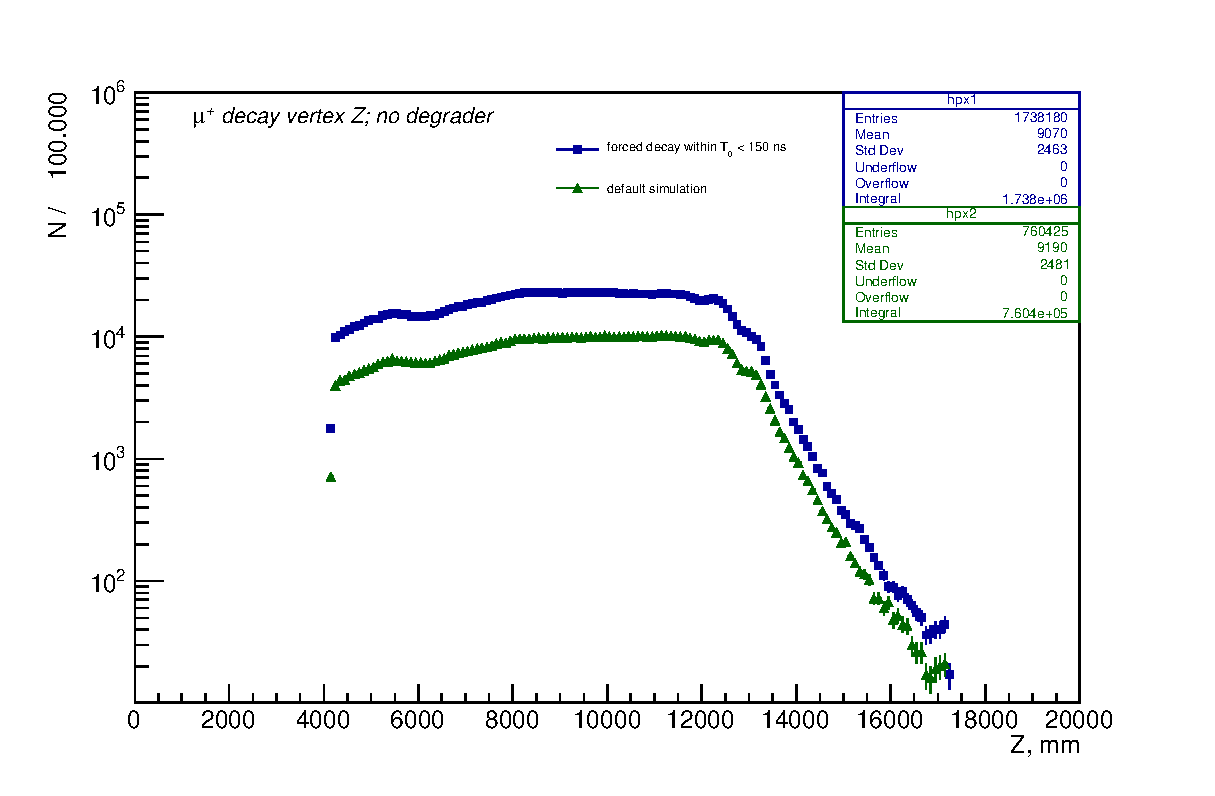
\includegraphics[width=0.55\textwidth]{pdf/figure_03401}
        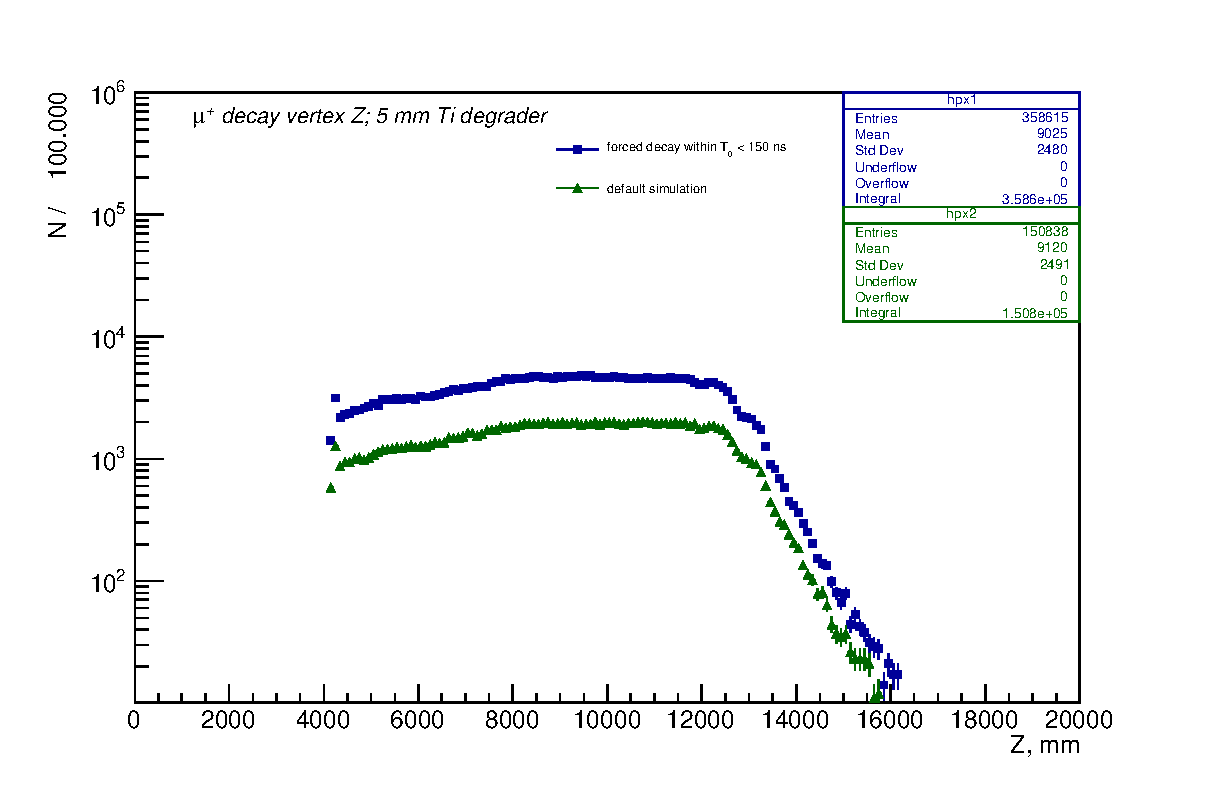
\includegraphics[width=0.55\textwidth]{pdf/figure_03451}
      }
    };
    % \node [text width=8cm, scale=1.0] at (14.5,0.5) {$\mu_B$, expected background mean};
    % \node [text width=8cm, scale=1.0, rotate={90}] at (1.5,7.5) { $S_{D}$, ``discovery'' signal strength  };
  \end{tikzpicture}
  \caption{
    \label{fig:pion_stop_time}
    Distributions of the Z-coordinates of mu+ vertices without the degrader (left)
    and for 5 mm Ti degrader (right)
  }
\end{figure}

\begin{figure}[H]
  \begin{tikzpicture}
    \node[anchor=south west,inner sep=0] at (0,0.) {
      % \node[shift={(0 cm,0.cm)},inner sep=0,rotate={90}] at (0,0) {}
      \makebox[\textwidth][c] {
        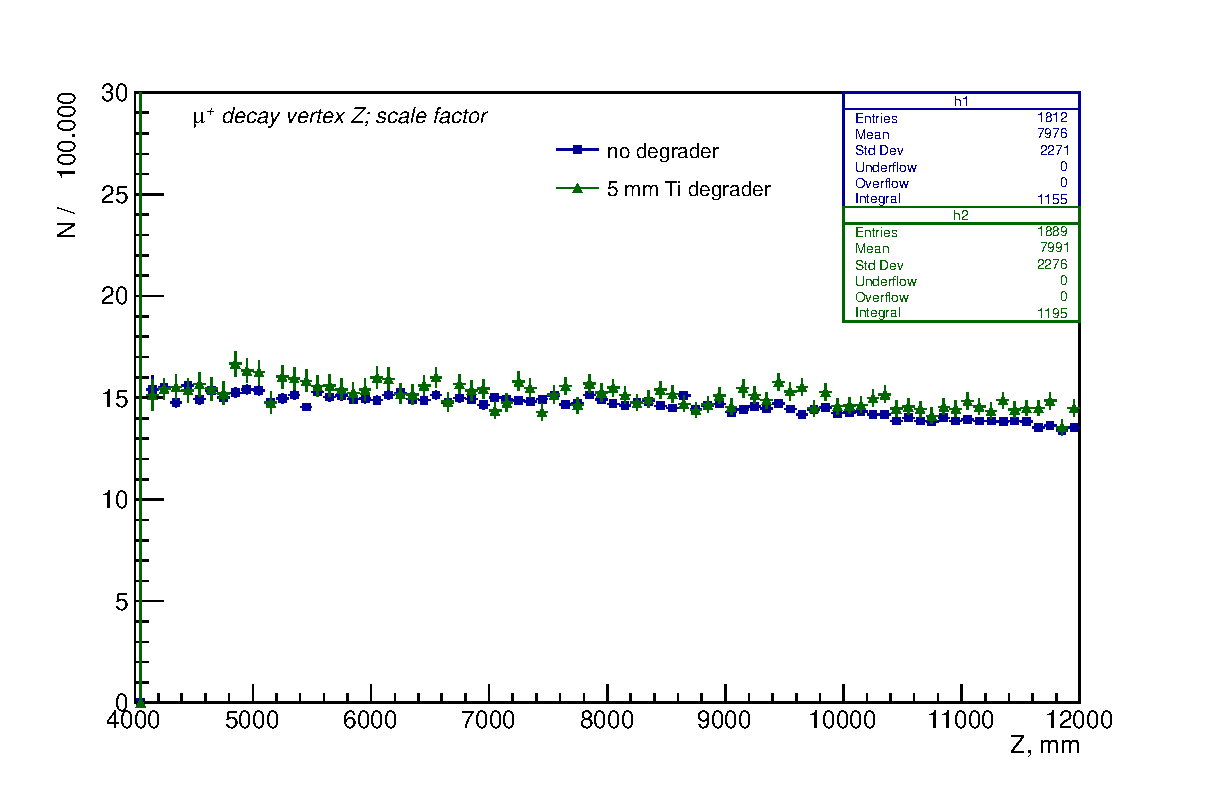
\includegraphics[width=0.8\textwidth]{pdf/figure_03701}
      }
    };
    % \node [text width=8cm, scale=1.0] at (14.5,0.5) {$\mu_B$, expected background mean};
    % \node [text width=8cm, scale=1.0, rotate={90}] at (1.5,7.5) { $S_{D}$, ``discovery'' signal strength  };
  \end{tikzpicture}
  \caption{
    \label{fig:pion_stop_time}
    The ratio of the Z vertex distributions - the scale factor
  }
\end{figure}


The scale factor coming out of the simulation is $SF = 15.0 \pm 0.5$ , consistent with the back-of-the-envelope
estimate of
$$
            SF = 1/(1 - exp^{-T_{max}/\tau}) = 15.15 ~~,
$$
where $T_{max} = 150$ ns and $\tau = 2197$ ns, the muon lifetime at rest.
Therefore constraining the muon proper decay time in the detector to 150 ns improves the simulation efficiency
by a factor of 15 w/o introducing extra event-dependent weights.

%%% Local Variables:
%%% mode: latex
%%% TeX-master: "mu2e-xxxxx"
%%% End:
